\documentclass[a4paper,10pt]{report}
\usepackage[utf8]{inputenc}
\usepackage[pdftex]{graphicx}
\usepackage{fancyhdr}
\usepackage{listings}
\usepackage[francais]{babel}
\usepackage{hyperref}
\usepackage{amsmath}

% Title Page
\title{IA01 : TP2}
\author{Par Camille Gerin-Roze et Thomas Perrin}



\renewcommand{\footrulewidth}{1pt}
\fancyfoot[C]{\textbf{\thepage}} 	
\fancyfoot[L]{}

\hypersetup{
	colorlinks=true,
	linkcolor=black
}

\begin{document}

\begin{titlepage}

\begin{flushright}
  
\includegraphics[scale = 0.2]{logo_utc.jpg}
\end{flushright}
\vspace*{5cm}

\newcommand{\HRule}{\rule{\linewidth}{0.5mm}} % Defines a new command for the horizontal lines, change thickness here
\center % Center everything on the page
 


%----------------------------------------------------------------------------------------
%	TITLE SECTION
%----------------------------------------------------------------------------------------

\HRule \\[0.4cm]
{ \LARGE \bfseries  IA01 : Rapport du TP2}\\[0.4cm] % Title of your document
\HRule \\[1.5cm]
 
%----------------------------------------------------------------------------------------
%	AUTHOR SECTION
%----------------------------------------------------------------------------------------
\begin{minipage}{0.4\textwidth}
\begin{flushleft} \large
\emph{Auteurs:}\\
Camille \textsc{Gerin-Roze} \newline
Thomas \textsc{Perrin} 
\end{flushleft}
\end{minipage}
~
\begin{minipage}{0.4\textwidth}

\end{minipage}\\[1.3cm]


{\large Le 15 Novembre 2015} % Date, change the \today to a set date if you want to be precise

\end{titlepage}
\tableofcontents
\chapter*{Introduction}

Le but de ce TP est de réfléchir à une recherche dans un espace d’états avec le langage Lisp. Au départ, nous effectuerons une recherche basique en profondeur,
pour ensuite considérer une heuristique afin d'optimiser cette recherche. 
Dans ce rapport, nous répondrons aux différentes questions posés et nous expliquerons de quel manière nous avons abordé les problèmes et pourquoi.
Nous utiliserons plusieurs fonctions dites « de service » :

\begin{itemize}
 \item get\_symbol : Permet d'obtenir le symbole à l'index en paramètre.
 \item myMember : Implémentation différente de la fonction member avec la fonction EQUAL au lieu de EQ.
 \item etat\_correct : Permet de déterminer si un état est correct en vérifiant la présence de A, B, C, D, que la structure soit de taille 4 et que A soit placé avant D.
 \end{itemize}



\chapter{Graphe d'états}

\begin{figure}[h!]
  \centering
 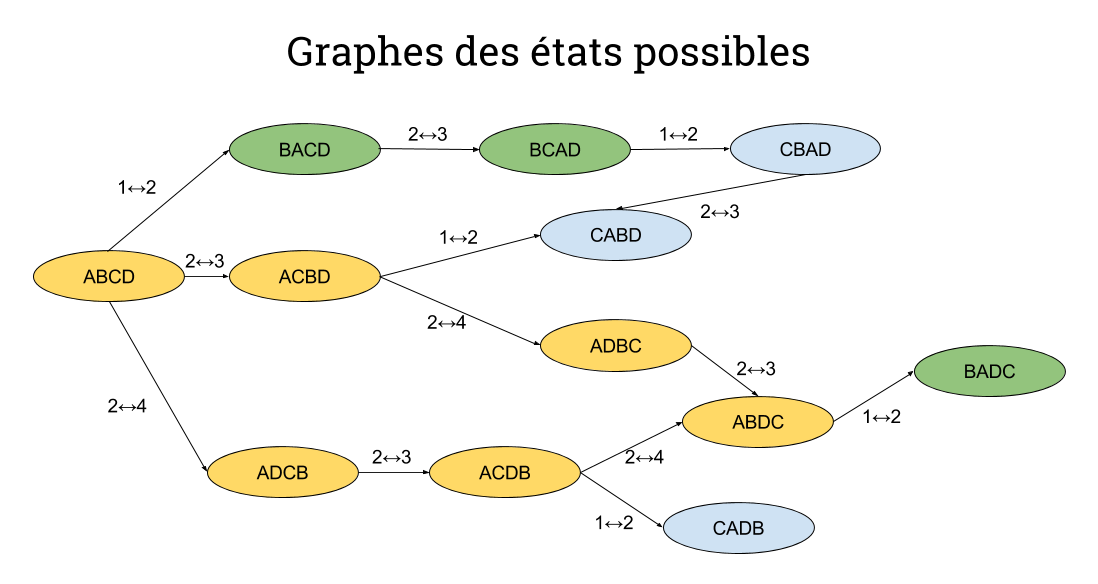
\includegraphics[scale=0.4]{Graphe_D_Etat.png}
 \caption{Graphe représentants les états et leurs successeurs}
\end{figure}

De base, seules trois actions sont possibles à chaque état. Ensuite, à chaque successeur, on retire la même action qui va uniquement revenir en arrière. De plus, certaines actions peuvent être interdites puisqu’ils modifieraient les pions dans un état non autorisé. Ainsi, ce graphe d’états permet de représenter clairement les différentes possibilités en indiquant unitairement chaque état.

\chapter{Successeurs d'un état}

  \section{La fonction echange(x,y)}
  La fonction echange reforme les 4 pions à partir d’une liste vide. A chaque itération, on ajoute le pion correspondant, mis à part lorsque l’on est aux deux index précisés en paramètre.  On vérifie ici uniquement que les deux index sont accessibles, on limitera les actions possibles dans la fonction successeurs.
  \section{La fonction successeurs}
  La fonction successeurs effectue les trois actions autorisés par l’énoncé sur l’état en paramètre : c’est-à-dire echange(1,2), echange(2,3) et echange(2,4). Si le successeur est valide (vérifié grâce à la fonction de service etat_correct), on l’ajoute à la liste des successeurs. Ainsi, on obtiendra une liste pouvant aller de 0 à 3 états.



\end{document}          
